\documentclass{standalone}
\usepackage{tikz}
\usetikzlibrary{patterns, positioning}

\begin{document}
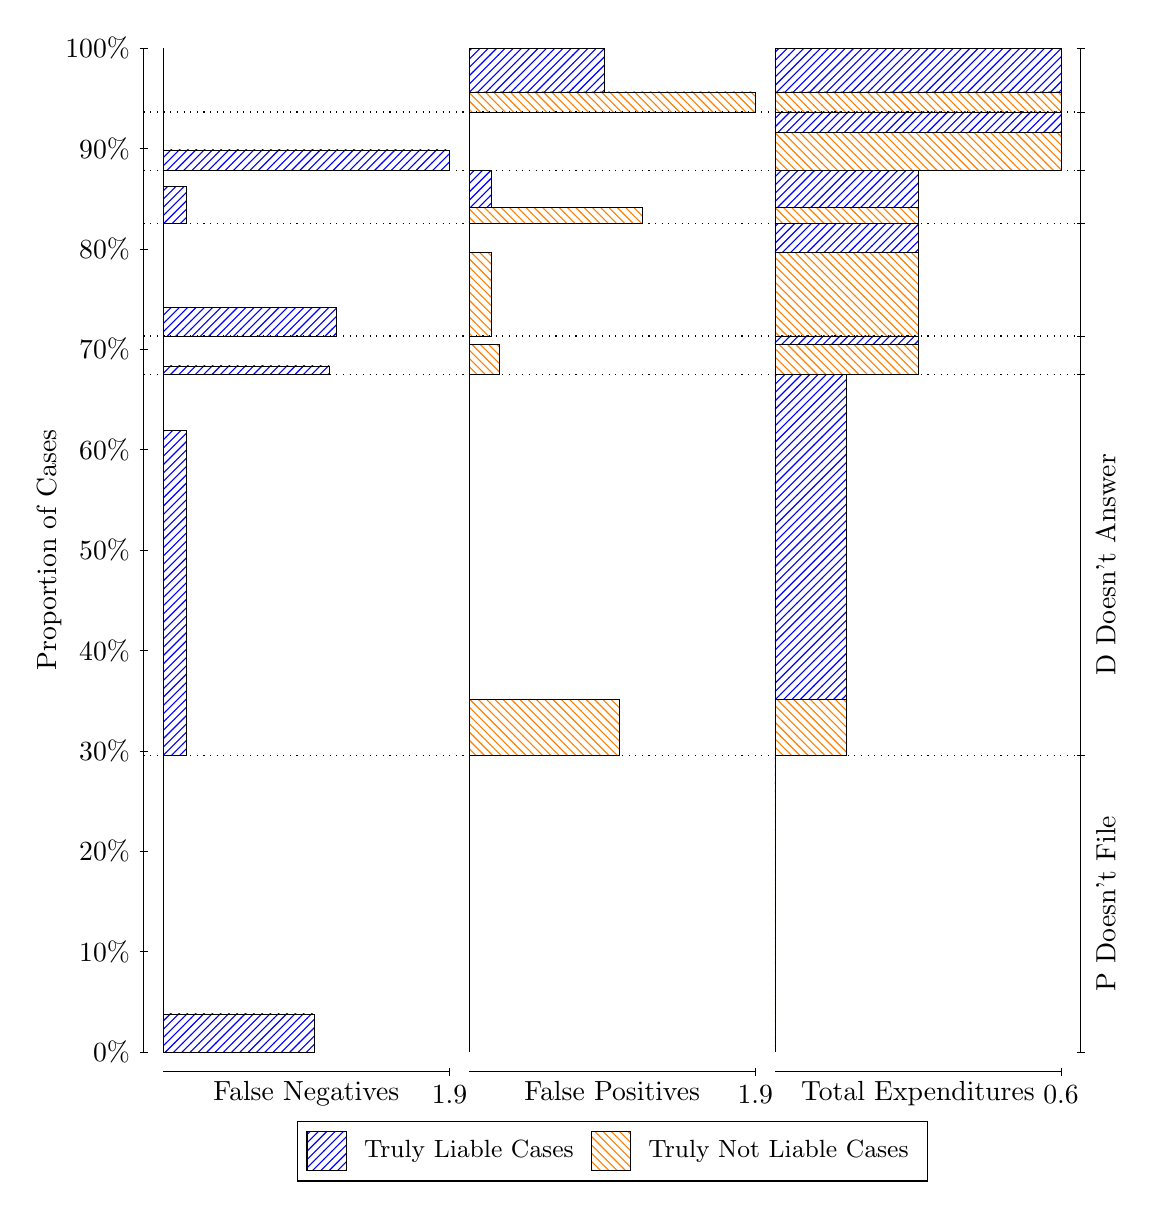
\begin{tikzpicture}
\draw[black, very thin] (1.5,1.75) -- (1.5,14.5);
\node[rotate=90, anchor=center] at (0.3, 8.125) {Proportion of Cases};
\draw[black, very thin] (1.45,1.75) -- (1.55,1.75);
\node[anchor=east] at (1.45, 1.75) {0\%};
\draw[black, very thin] (1.45,3.025) -- (1.55,3.025);
\node[anchor=east] at (1.45, 3.025) {10\%};
\draw[black, very thin] (1.45,4.3) -- (1.55,4.3);
\node[anchor=east] at (1.45, 4.3) {20\%};
\draw[black, very thin] (1.45,5.575) -- (1.55,5.575);
\node[anchor=east] at (1.45, 5.575) {30\%};
\draw[black, very thin] (1.45,6.85) -- (1.55,6.85);
\node[anchor=east] at (1.45, 6.85) {40\%};
\draw[black, very thin] (1.45,8.125) -- (1.55,8.125);
\node[anchor=east] at (1.45, 8.125) {50\%};
\draw[black, very thin] (1.45,9.4) -- (1.55,9.4);
\node[anchor=east] at (1.45, 9.4) {60\%};
\draw[black, very thin] (1.45,10.675) -- (1.55,10.675);
\node[anchor=east] at (1.45, 10.675) {70\%};
\draw[black, very thin] (1.45,11.95) -- (1.55,11.95);
\node[anchor=east] at (1.45, 11.95) {80\%};
\draw[black, very thin] (1.45,13.225) -- (1.55,13.225);
\node[anchor=east] at (1.45, 13.225) {90\%};
\draw[black, very thin] (1.45,14.5) -- (1.55,14.5);
\node[anchor=east] at (1.45, 14.5) {100\%};

\draw[black, very thin] (13.4,1.75) -- (13.4,14.5);
\draw[black, very thin] (13.35,1.75) -- (13.45,1.75);
\node[anchor=west] at (13.35, 1.75) {};
\draw[black, very thin] (13.35,5.5119) -- (13.45,5.5119);
\node[anchor=west] at (13.35, 5.5119) {};
\draw[black, very thin] (13.35,10.359) -- (13.45,10.359);
\node[anchor=west] at (13.35, 10.359) {};
\draw[black, very thin] (13.35,10.843) -- (13.45,10.843);
\node[anchor=west] at (13.35, 10.843) {};
\draw[black, very thin] (13.35,12.27) -- (13.45,12.27);
\node[anchor=west] at (13.35, 12.27) {};
\draw[black, very thin] (13.35,12.95) -- (13.45,12.95);
\node[anchor=west] at (13.35, 12.95) {};
\draw[black, very thin] (13.35,13.688) -- (13.45,13.688);
\node[anchor=west] at (13.35, 13.688) {};
\draw[black, very thin] (13.35,14.5) -- (13.45,14.5);
\node[anchor=west] at (13.35, 14.5) {};

\draw[black, very thin, pattern color=blue, pattern=north east lines] (1.75,1.75) rectangle (3.6623,2.2345);
\draw[black, very thin, pattern color=orange, pattern=north west lines] (1.75,2.2345) rectangle (1.75,5.5119);
\draw[black, very thin, pattern color=blue, pattern=north east lines] (1.75,5.5119) rectangle (2.0368,9.6455);
\draw[black, very thin, pattern color=orange, pattern=north west lines] (1.75,9.6455) rectangle (1.75,10.359);
\draw[black, very thin, pattern color=blue, pattern=north east lines] (1.75,10.359) rectangle (3.8535,10.462);
\draw[black, very thin, pattern color=orange, pattern=north west lines] (1.75,10.462) rectangle (1.75,10.843);
\draw[black, very thin, pattern color=blue, pattern=north east lines] (1.75,10.843) rectangle (3.9491,11.21);
\draw[black, very thin, pattern color=orange, pattern=north west lines] (1.75,11.21) rectangle (1.75,12.27);
\draw[black, very thin, pattern color=blue, pattern=north east lines] (1.75,12.27) rectangle (2.0368,12.744);
\draw[black, very thin, pattern color=orange, pattern=north west lines] (1.75,12.744) rectangle (1.75,12.95);
\draw[black, very thin, pattern color=blue, pattern=north east lines] (1.75,12.95) rectangle (5.3833,13.206);
\draw[black, very thin, pattern color=orange, pattern=north west lines] (1.75,13.206) rectangle (1.75,13.688);
\draw[black, very thin, pattern color=orange, pattern=north west lines] (1.75,13.688) rectangle (1.75,13.944);
\draw[black, very thin, pattern color=blue, pattern=north east lines] (1.75,13.944) rectangle (1.75,14.5);
\draw[black, very thin, pattern color=orange, pattern=north west lines] (5.6333,1.75) rectangle (5.6333,5.0274);
\draw[black, very thin, pattern color=blue, pattern=north east lines] (5.6333,5.0274) rectangle (5.6333,5.5119);
\draw[black, very thin, pattern color=orange, pattern=north west lines] (5.6333,5.5119) rectangle (7.5456,6.2249);
\draw[black, very thin, pattern color=blue, pattern=north east lines] (5.6333,6.2249) rectangle (5.6333,10.359);
\draw[black, very thin, pattern color=orange, pattern=north west lines] (5.6333,10.359) rectangle (6.0158,10.74);
\draw[black, very thin, pattern color=blue, pattern=north east lines] (5.6333,10.74) rectangle (5.6333,10.843);
\draw[black, very thin, pattern color=orange, pattern=north west lines] (5.6333,10.843) rectangle (5.9202,11.903);
\draw[black, very thin, pattern color=blue, pattern=north east lines] (5.6333,11.903) rectangle (5.6333,12.27);
\draw[black, very thin, pattern color=orange, pattern=north west lines] (5.6333,12.27) rectangle (7.8325,12.476);
\draw[black, very thin, pattern color=blue, pattern=north east lines] (5.6333,12.476) rectangle (5.9202,12.95);
\draw[black, very thin, pattern color=orange, pattern=north west lines] (5.6333,12.95) rectangle (5.6333,13.431);
\draw[black, very thin, pattern color=blue, pattern=north east lines] (5.6333,13.431) rectangle (5.6333,13.688);
\draw[black, very thin, pattern color=orange, pattern=north west lines] (5.6333,13.688) rectangle (9.2667,13.944);
\draw[black, very thin, pattern color=blue, pattern=north east lines] (5.6333,13.944) rectangle (7.3544,14.5);
\draw[black, very thin, pattern color=orange, pattern=north west lines] (9.5167,1.75) rectangle (9.5167,5.0274);
\draw[black, very thin, pattern color=blue, pattern=north east lines] (9.5167,5.0274) rectangle (9.5167,5.5119);
\draw[black, very thin, pattern color=orange, pattern=north west lines] (9.5167,5.5119) rectangle (10.425,6.2249);
\draw[black, very thin, pattern color=blue, pattern=north east lines] (9.5167,6.2249) rectangle (10.425,10.359);
\draw[black, very thin, pattern color=orange, pattern=north west lines] (9.5167,10.359) rectangle (11.333,10.74);
\draw[black, very thin, pattern color=blue, pattern=north east lines] (9.5167,10.74) rectangle (11.333,10.843);
\draw[black, very thin, pattern color=orange, pattern=north west lines] (9.5167,10.843) rectangle (11.333,11.903);
\draw[black, very thin, pattern color=blue, pattern=north east lines] (9.5167,11.903) rectangle (11.333,12.27);
\draw[black, very thin, pattern color=orange, pattern=north west lines] (9.5167,12.27) rectangle (11.333,12.476);
\draw[black, very thin, pattern color=blue, pattern=north east lines] (9.5167,12.476) rectangle (11.333,12.95);
\draw[black, very thin, pattern color=orange, pattern=north west lines] (9.5167,12.95) rectangle (13.15,13.431);
\draw[black, very thin, pattern color=blue, pattern=north east lines] (9.5167,13.431) rectangle (13.15,13.688);
\draw[black, very thin, pattern color=orange, pattern=north west lines] (9.5167,13.688) rectangle (13.15,13.944);
\draw[black, very thin, pattern color=blue, pattern=north east lines] (9.5167,13.944) rectangle (13.15,14.5);
\draw[black, dotted] (1.5,5.5119) -- (13.4,5.5119);
\draw[black, dotted] (1.5,10.359) -- (13.4,10.359);
\draw[black, dotted] (1.5,10.843) -- (13.4,10.843);
\draw[black, dotted] (1.5,12.27) -- (13.4,12.27);
\draw[black, dotted] (1.5,12.95) -- (13.4,12.95);
\draw[black, dotted] (1.5,13.688) -- (13.4,13.688);
\draw[black, very thin] (1.75,1.5) -- (5.3833,1.5);
\node[anchor=north] at (3.5667, 1.5) {False Negatives};
\draw[black, very thin] (5.3833,1.45) -- (5.3833,1.55);
\node[anchor=north] at (5.3833, 1.45) {1.9};

\draw[black, very thin] (5.6333,1.5) -- (9.2667,1.5);
\node[anchor=north] at (7.45, 1.5) {False Positives};
\draw[black, very thin] (9.2667,1.45) -- (9.2667,1.55);
\node[anchor=north] at (9.2667, 1.45) {1.9};

\draw[black, very thin] (9.5167,1.5) -- (13.15,1.5);
\node[anchor=north] at (11.333, 1.5) {Total Expenditures};
\draw[black, very thin] (13.15,1.45) -- (13.15,1.55);
\node[anchor=north] at (13.15, 1.45) {0.6};

\node[black, centered, rotate=90] at (13.72, 3.6309) {P Doesn't File};
\node[black, centered, rotate=90] at (13.72, 7.9352) {D Doesn't Answer};






\draw (7.449999999999999,1.5) node[draw=none] (baseCoordinate) {};
\begin{scope}[align=center]
        \matrix[scale=0.5, draw=black, below=0.5cm of baseCoordinate, nodes={draw}, column sep=0.1cm]{
            \node[rectangle, draw, minimum width=0.5cm, minimum height=0.5cm, pattern=north east lines, pattern color=blue] {}; &
            \node[draw=none, font=\small] (B) {Truly Liable Cases}; &
            \node[rectangle, draw, minimum width=0.5cm, minimum height=0.5cm, pattern=north west lines, pattern color=orange] {}; &
            \node[draw=none, font=\small] (B) {Truly Not Liable Cases}; \\
            };
\end{scope}

\end{tikzpicture}
\end{document}